% Options for packages loaded elsewhere
\PassOptionsToPackage{unicode}{hyperref}
\PassOptionsToPackage{hyphens}{url}
\PassOptionsToPackage{dvipsnames,svgnames,x11names}{xcolor}
%
\documentclass[
  letterpaper,
  DIV=11,
  numbers=noendperiod]{scrartcl}

\usepackage{amsmath,amssymb}
\usepackage{iftex}
\ifPDFTeX
  \usepackage[T1]{fontenc}
  \usepackage[utf8]{inputenc}
  \usepackage{textcomp} % provide euro and other symbols
\else % if luatex or xetex
  \usepackage{unicode-math}
  \defaultfontfeatures{Scale=MatchLowercase}
  \defaultfontfeatures[\rmfamily]{Ligatures=TeX,Scale=1}
\fi
\usepackage{lmodern}
\ifPDFTeX\else  
    % xetex/luatex font selection
\fi
% Use upquote if available, for straight quotes in verbatim environments
\IfFileExists{upquote.sty}{\usepackage{upquote}}{}
\IfFileExists{microtype.sty}{% use microtype if available
  \usepackage[]{microtype}
  \UseMicrotypeSet[protrusion]{basicmath} % disable protrusion for tt fonts
}{}
\makeatletter
\@ifundefined{KOMAClassName}{% if non-KOMA class
  \IfFileExists{parskip.sty}{%
    \usepackage{parskip}
  }{% else
    \setlength{\parindent}{0pt}
    \setlength{\parskip}{6pt plus 2pt minus 1pt}}
}{% if KOMA class
  \KOMAoptions{parskip=half}}
\makeatother
\usepackage{xcolor}
\setlength{\emergencystretch}{3em} % prevent overfull lines
\setcounter{secnumdepth}{-\maxdimen} % remove section numbering
% Make \paragraph and \subparagraph free-standing
\makeatletter
\ifx\paragraph\undefined\else
  \let\oldparagraph\paragraph
  \renewcommand{\paragraph}{
    \@ifstar
      \xxxParagraphStar
      \xxxParagraphNoStar
  }
  \newcommand{\xxxParagraphStar}[1]{\oldparagraph*{#1}\mbox{}}
  \newcommand{\xxxParagraphNoStar}[1]{\oldparagraph{#1}\mbox{}}
\fi
\ifx\subparagraph\undefined\else
  \let\oldsubparagraph\subparagraph
  \renewcommand{\subparagraph}{
    \@ifstar
      \xxxSubParagraphStar
      \xxxSubParagraphNoStar
  }
  \newcommand{\xxxSubParagraphStar}[1]{\oldsubparagraph*{#1}\mbox{}}
  \newcommand{\xxxSubParagraphNoStar}[1]{\oldsubparagraph{#1}\mbox{}}
\fi
\makeatother

\usepackage{color}
\usepackage{fancyvrb}
\newcommand{\VerbBar}{|}
\newcommand{\VERB}{\Verb[commandchars=\\\{\}]}
\DefineVerbatimEnvironment{Highlighting}{Verbatim}{commandchars=\\\{\}}
% Add ',fontsize=\small' for more characters per line
\usepackage{framed}
\definecolor{shadecolor}{RGB}{241,243,245}
\newenvironment{Shaded}{\begin{snugshade}}{\end{snugshade}}
\newcommand{\AlertTok}[1]{\textcolor[rgb]{0.68,0.00,0.00}{#1}}
\newcommand{\AnnotationTok}[1]{\textcolor[rgb]{0.37,0.37,0.37}{#1}}
\newcommand{\AttributeTok}[1]{\textcolor[rgb]{0.40,0.45,0.13}{#1}}
\newcommand{\BaseNTok}[1]{\textcolor[rgb]{0.68,0.00,0.00}{#1}}
\newcommand{\BuiltInTok}[1]{\textcolor[rgb]{0.00,0.23,0.31}{#1}}
\newcommand{\CharTok}[1]{\textcolor[rgb]{0.13,0.47,0.30}{#1}}
\newcommand{\CommentTok}[1]{\textcolor[rgb]{0.37,0.37,0.37}{#1}}
\newcommand{\CommentVarTok}[1]{\textcolor[rgb]{0.37,0.37,0.37}{\textit{#1}}}
\newcommand{\ConstantTok}[1]{\textcolor[rgb]{0.56,0.35,0.01}{#1}}
\newcommand{\ControlFlowTok}[1]{\textcolor[rgb]{0.00,0.23,0.31}{\textbf{#1}}}
\newcommand{\DataTypeTok}[1]{\textcolor[rgb]{0.68,0.00,0.00}{#1}}
\newcommand{\DecValTok}[1]{\textcolor[rgb]{0.68,0.00,0.00}{#1}}
\newcommand{\DocumentationTok}[1]{\textcolor[rgb]{0.37,0.37,0.37}{\textit{#1}}}
\newcommand{\ErrorTok}[1]{\textcolor[rgb]{0.68,0.00,0.00}{#1}}
\newcommand{\ExtensionTok}[1]{\textcolor[rgb]{0.00,0.23,0.31}{#1}}
\newcommand{\FloatTok}[1]{\textcolor[rgb]{0.68,0.00,0.00}{#1}}
\newcommand{\FunctionTok}[1]{\textcolor[rgb]{0.28,0.35,0.67}{#1}}
\newcommand{\ImportTok}[1]{\textcolor[rgb]{0.00,0.46,0.62}{#1}}
\newcommand{\InformationTok}[1]{\textcolor[rgb]{0.37,0.37,0.37}{#1}}
\newcommand{\KeywordTok}[1]{\textcolor[rgb]{0.00,0.23,0.31}{\textbf{#1}}}
\newcommand{\NormalTok}[1]{\textcolor[rgb]{0.00,0.23,0.31}{#1}}
\newcommand{\OperatorTok}[1]{\textcolor[rgb]{0.37,0.37,0.37}{#1}}
\newcommand{\OtherTok}[1]{\textcolor[rgb]{0.00,0.23,0.31}{#1}}
\newcommand{\PreprocessorTok}[1]{\textcolor[rgb]{0.68,0.00,0.00}{#1}}
\newcommand{\RegionMarkerTok}[1]{\textcolor[rgb]{0.00,0.23,0.31}{#1}}
\newcommand{\SpecialCharTok}[1]{\textcolor[rgb]{0.37,0.37,0.37}{#1}}
\newcommand{\SpecialStringTok}[1]{\textcolor[rgb]{0.13,0.47,0.30}{#1}}
\newcommand{\StringTok}[1]{\textcolor[rgb]{0.13,0.47,0.30}{#1}}
\newcommand{\VariableTok}[1]{\textcolor[rgb]{0.07,0.07,0.07}{#1}}
\newcommand{\VerbatimStringTok}[1]{\textcolor[rgb]{0.13,0.47,0.30}{#1}}
\newcommand{\WarningTok}[1]{\textcolor[rgb]{0.37,0.37,0.37}{\textit{#1}}}

\providecommand{\tightlist}{%
  \setlength{\itemsep}{0pt}\setlength{\parskip}{0pt}}\usepackage{longtable,booktabs,array}
\usepackage{calc} % for calculating minipage widths
% Correct order of tables after \paragraph or \subparagraph
\usepackage{etoolbox}
\makeatletter
\patchcmd\longtable{\par}{\if@noskipsec\mbox{}\fi\par}{}{}
\makeatother
% Allow footnotes in longtable head/foot
\IfFileExists{footnotehyper.sty}{\usepackage{footnotehyper}}{\usepackage{footnote}}
\makesavenoteenv{longtable}
\usepackage{graphicx}
\makeatletter
\def\maxwidth{\ifdim\Gin@nat@width>\linewidth\linewidth\else\Gin@nat@width\fi}
\def\maxheight{\ifdim\Gin@nat@height>\textheight\textheight\else\Gin@nat@height\fi}
\makeatother
% Scale images if necessary, so that they will not overflow the page
% margins by default, and it is still possible to overwrite the defaults
% using explicit options in \includegraphics[width, height, ...]{}
\setkeys{Gin}{width=\maxwidth,height=\maxheight,keepaspectratio}
% Set default figure placement to htbp
\makeatletter
\def\fps@figure{htbp}
\makeatother

\usepackage{graphicx}
\DeclareGraphicsExtensions{.pdf,.png,.jpg,.jpeg}
\KOMAoption{captions}{tableheading}
\makeatletter
\@ifpackageloaded{caption}{}{\usepackage{caption}}
\AtBeginDocument{%
\ifdefined\contentsname
  \renewcommand*\contentsname{Table of contents}
\else
  \newcommand\contentsname{Table of contents}
\fi
\ifdefined\listfigurename
  \renewcommand*\listfigurename{List of Figures}
\else
  \newcommand\listfigurename{List of Figures}
\fi
\ifdefined\listtablename
  \renewcommand*\listtablename{List of Tables}
\else
  \newcommand\listtablename{List of Tables}
\fi
\ifdefined\figurename
  \renewcommand*\figurename{Figure}
\else
  \newcommand\figurename{Figure}
\fi
\ifdefined\tablename
  \renewcommand*\tablename{Table}
\else
  \newcommand\tablename{Table}
\fi
}
\@ifpackageloaded{float}{}{\usepackage{float}}
\floatstyle{ruled}
\@ifundefined{c@chapter}{\newfloat{codelisting}{h}{lop}}{\newfloat{codelisting}{h}{lop}[chapter]}
\floatname{codelisting}{Listing}
\newcommand*\listoflistings{\listof{codelisting}{List of Listings}}
\makeatother
\makeatletter
\makeatother
\makeatletter
\@ifpackageloaded{caption}{}{\usepackage{caption}}
\@ifpackageloaded{subcaption}{}{\usepackage{subcaption}}
\makeatother

\ifLuaTeX
  \usepackage{selnolig}  % disable illegal ligatures
\fi
\usepackage{bookmark}

\IfFileExists{xurl.sty}{\usepackage{xurl}}{} % add URL line breaks if available
\urlstyle{same} % disable monospaced font for URLs
\hypersetup{
  pdftitle={Ch4 Lecture 1},
  colorlinks=true,
  linkcolor={blue},
  filecolor={Maroon},
  citecolor={Blue},
  urlcolor={Blue},
  pdfcreator={LaTeX via pandoc}}


\title{Ch4 Lecture 1}
\author{}
\date{}

\begin{document}
\maketitle


\section{\texorpdfstring{\emph{Planes, Hyperplanes, and
Projections}}{Planes, Hyperplanes, and Projections}}\label{planes-hyperplanes-and-projections}

Geometry of planes in \(\mathbb{R}^n\): equations, normals, distances,
and projections onto planes.

. . .

\subsection{\texorpdfstring{\emph{Why planes and
hyperplanes?}}{Why planes and hyperplanes?}}\label{why-planes-and-hyperplanes}

\begin{itemize}
\tightlist
\item
  Planes and hyperplanes are the solution sets of a single linear
  equation \(\mathbf{a} \cdot \mathbf{x} = b\) (vector \(\mathbf{a}\),
  scalar \(b\)).
\item
  Projections onto planes are the core of least-squares fitting and many
  applications.
\end{itemize}

. . .

\subsection{\texorpdfstring{\emph{The plane through the
origin}}{The plane through the origin}}\label{the-plane-through-the-origin}

A plane through the origin is the set of all vectors \(\vec x\) such
that \(\vec a \cdot \vec x = 0\), where the nonzero vector \(\vec a\) is
a \textbf{normal vector} to the plane (we often take \(\vec a\) of unit
length).

. . .

\subsection{\texorpdfstring{\emph{Finding the normal vector when we know
two vectors in the
plane}}{Finding the normal vector when we know two vectors in the plane}}\label{finding-the-normal-vector-when-we-know-two-vectors-in-the-plane}

For \(\mathbb{R}^3\), we can find the normal vector by taking the cross
product of two vectors in the plane.

Let \(\mathbf{i}, \mathbf{j}\), and \(\mathbf{k}\) represent the
standard basis \(\mathbf{e}_{1}, \mathbf{e}_{2}, \mathbf{e}_{3}\).

\[
\mathbf{u} \times \mathbf{v}=\left(u_{2} v_{3}-u_{3} v_{2}\right) \mathbf{i}+\left(u_{3} v_{1}-u_{1} v_{3}\right) \mathbf{j}+\left(u_{1} v_{2}-u_{2} v_{1}\right) \mathbf{k}=\left|\begin{array}{ccc}
\mathbf{i} & \mathbf{j} & \mathbf{k} \\
u_{1} & u_{2} & u_{3} \\
v_{1} & v_{2} & v_{3}
\end{array}\right|
\]

. . .

The cross product is orthogonal to both \(\mathbf{u}\) and
\(\mathbf{v}\): \(\mathbf{u} \cdot (\mathbf{u} \times \mathbf{v})=0\)
and \(\mathbf{v} \cdot (\mathbf{u} \times \mathbf{v})=0\).

. . .

We can use the cross product to find the normal vector to the plane by
taking the cross product of two vectors in the plane.

\subsection{\texorpdfstring{\emph{Finding the normal vector from the
equation of the
plane}}{Finding the normal vector from the equation of the plane}}\label{finding-the-normal-vector-from-the-equation-of-the-plane}

If the plane is specified by \(ax + by + cz = d\), then a normal vector
is \(\vec a = (a, b, c)\).

. . .

\textbf{Check (optional verification):}

\begin{enumerate}
\def\labelenumi{\arabic{enumi}.}
\tightlist
\item
  Find three points on the plane: e.g.~\((0, 0, d/c)\), \((0, d/b, 0)\),
  \((d/a, 0, 0)\) (when \(a,b,c \neq 0\)).
\item
  Form two displacement vectors in the plane,
  e.g.~\(\vec u = (0, d/b, -d/c)\) and \(\vec v = (d/a, 0, -d/c)\).
\end{enumerate}

. . .

\subsection{\texorpdfstring{\emph{Verifying the normal from
\(ax+by+cz=d\)}}{Verifying the normal from ax+by+cz=d}}\label{verifying-the-normal-from-axbyczd}

Take the cross product \(\vec u \times \vec v\):

\[
\begin{aligned}
\vec u \times \vec v
&= \left|\begin{array}{ccc}
\mathbf{i} & \mathbf{j} & \mathbf{k} \\
0 & d/b & -d/c \\
d/a & 0 & -d/c
\end{array}\right| \\
&= -\frac{d^2}{bc} \mathbf{i} + \frac{d^2}{ac} \mathbf{j} - \frac{d^2}{ab} \mathbf{k}
= -\frac{d^2}{abc} \left( a \mathbf{i} - b \mathbf{j} + c \mathbf{k} \right)
\end{aligned}
\]

This is parallel to \(\vec{a} = (a, b, c)\).

. . .

\subsection{\texorpdfstring{\emph{Distances from the
plane}}{Distances from the plane}}\label{distances-from-the-plane}

The distance from a point \(\vec x\) to the plane
\(\vec a \cdot \vec x = 0\) is the scalar projection of \(\vec x\) onto
the normal:

\begin{itemize}
\tightlist
\item
  If \(\vec a\) is unit length: distance \(= |\vec a \cdot \vec x|\).
\item
  If not: distance \(= |\vec a \cdot \vec x| / \|\vec a\|\).
\end{itemize}

. . .

\subsection{\texorpdfstring{\emph{Closest point on the plane (through
the
origin)}}{Closest point on the plane (through the origin)}}\label{closest-point-on-the-plane-through-the-origin}

The displacement from \(\vec x\) to the closest point on the plane has
length \(|\vec a \cdot \vec x|/\|\vec a\|\) and direction along
\(\vec a\).

. . .

\subsection{\texorpdfstring{\emph{Projection onto the plane (through the
origin)}}{Projection onto the plane (through the origin)}}\label{projection-onto-the-plane-through-the-origin}

The closest point on the plane to \(\vec x\) is
\(\vec x - \vec a (\vec x \cdot \vec a)/\|\vec a\|^2\) --- i.e.,
\(\vec x\) minus the projection of \(\vec x\) onto \(\vec a\).

. . .

\subsection{\texorpdfstring{\emph{A plane not at the
origin}}{A plane not at the origin}}\label{a-plane-not-at-the-origin}

A plane displaced from the origin can be described by a normal
\(\vec a\) and a scalar \(q\): the plane is displaced by \(q \vec a\)
from the origin.

. . .

\subsection{\texorpdfstring{\emph{Equation of the displaced
plane}}{Equation of the displaced plane}}\label{equation-of-the-displaced-plane}

Points \(\vec x\) on the plane satisfy \(\vec a \cdot \vec x = q\) (with
\(\vec a\) unit length, \(q\) is the signed distance of the plane from
the origin).

. . .

\subsection{\texorpdfstring{\emph{Hyperplane}}{Hyperplane}}\label{hyperplane}

A \textbf{hyperplane} in \(\mathbb{R}^{n}\) is the set of all
\(\mathbf{x} \in \mathbb{R}^{n}\) such that
\(\mathbf{a} \cdot \mathbf{x}=b\), where the nonzero vector
\(\mathbf{a} \in \mathbb{R}^{n}\) and scalar \(b\) are given.

. . .

Let \(H\) be the hyperplane in \(\mathbb{R}^{n}\) defined by
\(\mathbf{a} \cdot \mathbf{x}=b\) and let \(\mathbf{x}_{*} \in H\). Then

\begin{enumerate}
\def\labelenumi{(\arabic{enumi})}
\item
  \(\mathbf{a}^{\perp}=\{\mathbf{y} \in \mathbb{R}^{n} \mid \mathbf{a} \cdot \mathbf{y}=0\}\)
  is a subspace of \(\mathbb{R}^{n}\) of dimension \(n-1\).
\item
  \(H=\mathbf{x}_{*}+\mathbf{a}^{\perp}=\{\mathbf{x}_{*}+\mathbf{y} \mid \mathbf{y} \in \mathbf{a}^{\perp}\}\).
\end{enumerate}

. . .

\subsection{\texorpdfstring{\emph{Example: plane through three
points}}{Example: plane through three points}}\label{example-plane-through-three-points}

Find an equation that defines the plane containing the three
(noncollinear) points \(P, Q\), and \(R\) with coordinates \((1,0,2)\),
\((2,1,0)\), and \((3,1,1)\), respectively.

. . .

\[
\begin{aligned}
\overrightarrow{P Q}&=(2,1,0)-(1,0,2)=(1,1,-2) \\
\overrightarrow{P R}&=(3,1,1)-(1,0,2)=(2,1,-1)
\end{aligned}
\]

. . .

\[
\mathbf{u} \times \mathbf{v}=\left|\begin{array}{ccc}
\mathbf{i} & \mathbf{j} & \mathbf{k} \\
1 & 1 & -2 \\
2 & 1 & -1
\end{array}\right|=\mathbf{i}-3 \mathbf{j}-\mathbf{k}
\]

. . .

The normal vector is \(\mathbf{a}=(1,-3,-1)\).

. . .

The equation of the plane is \(\mathbf{a} \cdot \mathbf{x}=b\). Using
\(P\):
\(b=\mathbf{a} \cdot \mathbf{P}=(1,-3,-1) \cdot (1,0,2)=1+0-2=-1\).

. . .

So the plane is \(x - 3y - z = -1\).

\subsection{\texorpdfstring{\emph{Projections to the displaced
plane}}{Projections to the displaced plane}}\label{projections-to-the-displaced-plane}

The closest point on the hyperplane \(\vec a \cdot \vec x = q\) to a
point \(\vec x\) is \(\vec x - \vec a (\vec a \cdot \vec x - q)\) (for
unit \(\vec a\)).

. . .

\subsection{\texorpdfstring{\emph{Summary: planes and
projections}}{Summary: planes and projections}}\label{summary-planes-and-projections}

\begin{itemize}
\tightlist
\item
  Plane through the origin: \(\vec a \cdot \vec x = 0\).
\item
  Plane displaced: \(\vec a \cdot \vec x = q\).
\item
  Scalar projection of \(\vec x\) onto \(\vec a\):
  \(\vec a \cdot \vec x / \|\vec a\|\).
\item
  Vector projection of \(\vec x\) onto \(\vec a\):
  \(\frac{\vec a}{\|\vec a\|} \frac{\vec a \cdot \vec x}{\|\vec a\|}\).
\item
  Projection of \(\vec x\) onto the plane \(\vec a \cdot \vec x = q\):
  \(\vec x - \vec a (\vec a \cdot \vec x - q)\).
\end{itemize}

. . .

\subsection{\texorpdfstring{\emph{Projection formula for
vectors}}{Projection formula for vectors}}\label{projection-formula-for-vectors}

Let \(\mathbf{u}\) and \(\mathbf{v}\) be vectors,
\(\mathbf{v} \neq \mathbf{0}\).

\[
\mathbf{p}=\frac{\mathbf{v} \cdot \mathbf{u}}{\mathbf{v} \cdot \mathbf{v}} \mathbf{v} \quad \text{and} \quad \mathbf{q}=\mathbf{u}-\mathbf{p}
\]

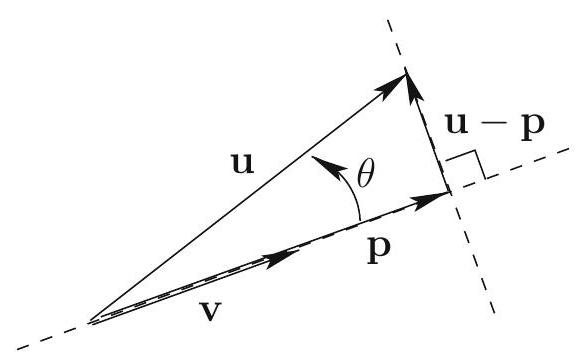
\includegraphics{images/day_9_fig1.jpg}

. . .

Then \(\mathbf{p}\) is \textbf{parallel} to \(\mathbf{v}\),
\(\mathbf{q}\) is \textbf{orthogonal} to \(\mathbf{v}\), and
\(\mathbf{u}=\mathbf{p}+\mathbf{q}\).

. . .

We write
\(\operatorname{proj}_{\mathbf{v}} \mathbf{u}=\frac{\mathbf{v} \cdot \mathbf{u}}{\mathbf{v} \cdot \mathbf{v}} \mathbf{v}\)
and
\(\operatorname{orth}_{\mathbf{v}} \mathbf{u}=\mathbf{u}-\operatorname{proj}_{\mathbf{v}} \mathbf{u}\).

. . .

\subsection{\texorpdfstring{\emph{Skills: Planes and
Projections}}{Skills: Planes and Projections}}\label{skills-planes-and-projections}

\begin{itemize}
\tightlist
\item
  Write the equation of a plane (through the origin or displaced) using
  a normal vector.
\item
  Find a normal to a plane from two vectors in the plane (cross product
  in \(\mathbb{R}^3\)) or from \(ax+by+cz=d\).
\item
  Compute distance from a point to a plane and the projection of a point
  onto a plane.
\item
  Use \(\operatorname{proj}_{\mathbf{v}} \mathbf{u}\) and
  \(\operatorname{orth}_{\mathbf{v}} \mathbf{u}\).
\end{itemize}

\section{\texorpdfstring{\emph{Fundamental Subspaces
(Pictures)}}{Fundamental Subspaces (Pictures)}}\label{fundamental-subspaces-pictures}

Geometric view of column space, row space, and null space in low
dimensions---and how that connects to least squares.

. . .

\subsection{\texorpdfstring{\emph{Why the pictures
matter}}{Why the pictures matter}}\label{why-the-pictures-matter}

\begin{itemize}
\tightlist
\item
  \textbf{Consistency of \(A\mathbf{x}=\mathbf{b}\):} solvable exactly
  when \(\mathbf{b} \in \mathcal{C}(A)\) (the ``reachable'' set).
\item
  \textbf{Least squares:} when \(\mathbf{b} \notin \mathcal{C}(A)\), we
  find the \textbf{closest point} in \(\mathcal{C}(A)\) to
  \(\mathbf{b}\) (projection onto the column space).
\item
  Seeing \(\mathcal{C}(A)\) as a line or plane makes this concrete.
\end{itemize}

. . .

\subsection{\texorpdfstring{\emph{When is the column space a
plane?}}{When is the column space a plane?}}\label{when-is-the-column-space-a-plane}

In \(\mathbb{R}^3\), the dimension of \(\mathcal{C}(A)\) equals the
\textbf{rank} \(r\) of \(A\):

\begin{itemize}
\tightlist
\item
  \textbf{Rank 1:} \(\mathcal{C}(A)\) is a \textbf{line} (all columns
  are multiples of one vector).
\item
  \textbf{Rank 2:} \(\mathcal{C}(A)\) is a \textbf{plane} (span of two
  independent columns).
\item
  \textbf{Rank 3:} \(\mathcal{C}(A)\) is \textbf{all of
  \(\mathbb{R}^3\)}.
\end{itemize}

. . .

\begin{Shaded}
\begin{Highlighting}[]
\ImportTok{import}\NormalTok{ plotly.graph\_objects }\ImportTok{as}\NormalTok{ go}
\ImportTok{import}\NormalTok{ numpy }\ImportTok{as}\NormalTok{ np}

\KeywordTok{def}\NormalTok{ add\_plane\_through\_origin(fig, v1, v2, name, color}\OperatorTok{=}\StringTok{\textquotesingle{}lightblue\textquotesingle{}}\NormalTok{, opacity}\OperatorTok{=}\FloatTok{0.6}\NormalTok{):}
    \CommentTok{"""Add a plane span(v1,v2) as a surface."""}
\NormalTok{    s }\OperatorTok{=}\NormalTok{ np.linspace(}\OperatorTok{{-}}\DecValTok{1}\NormalTok{, }\DecValTok{1}\NormalTok{, }\DecValTok{15}\NormalTok{)}
\NormalTok{    t }\OperatorTok{=}\NormalTok{ np.linspace(}\OperatorTok{{-}}\DecValTok{1}\NormalTok{, }\DecValTok{1}\NormalTok{, }\DecValTok{15}\NormalTok{)}
\NormalTok{    S, T }\OperatorTok{=}\NormalTok{ np.meshgrid(s, t)}
\NormalTok{    X }\OperatorTok{=}\NormalTok{ S }\OperatorTok{*}\NormalTok{ v1[}\DecValTok{0}\NormalTok{] }\OperatorTok{+}\NormalTok{ T }\OperatorTok{*}\NormalTok{ v2[}\DecValTok{0}\NormalTok{]}
\NormalTok{    Y }\OperatorTok{=}\NormalTok{ S }\OperatorTok{*}\NormalTok{ v1[}\DecValTok{1}\NormalTok{] }\OperatorTok{+}\NormalTok{ T }\OperatorTok{*}\NormalTok{ v2[}\DecValTok{1}\NormalTok{]}
\NormalTok{    Z }\OperatorTok{=}\NormalTok{ S }\OperatorTok{*}\NormalTok{ v1[}\DecValTok{2}\NormalTok{] }\OperatorTok{+}\NormalTok{ T }\OperatorTok{*}\NormalTok{ v2[}\DecValTok{2}\NormalTok{]}
\NormalTok{    fig.add\_trace(go.Surface(x}\OperatorTok{=}\NormalTok{X, y}\OperatorTok{=}\NormalTok{Y, z}\OperatorTok{=}\NormalTok{Z, name}\OperatorTok{=}\NormalTok{name, colorscale}\OperatorTok{=}\NormalTok{[[}\DecValTok{0}\NormalTok{, color], [}\DecValTok{1}\NormalTok{, color]], opacity}\OperatorTok{=}\NormalTok{opacity, showscale}\OperatorTok{=}\VariableTok{False}\NormalTok{))}

\KeywordTok{def}\NormalTok{ add\_line\_through\_origin(fig, v, name, color}\OperatorTok{=}\StringTok{\textquotesingle{}red\textquotesingle{}}\NormalTok{, width}\OperatorTok{=}\DecValTok{4}\NormalTok{):}
    \CommentTok{"""Add a line span(v) as a segment."""}
\NormalTok{    scale }\OperatorTok{=} \FloatTok{1.2}
\NormalTok{    fig.add\_trace(go.Scatter3d(x}\OperatorTok{=}\NormalTok{[}\OperatorTok{{-}}\NormalTok{scale}\OperatorTok{*}\NormalTok{v[}\DecValTok{0}\NormalTok{], scale}\OperatorTok{*}\NormalTok{v[}\DecValTok{0}\NormalTok{]], y}\OperatorTok{=}\NormalTok{[}\OperatorTok{{-}}\NormalTok{scale}\OperatorTok{*}\NormalTok{v[}\DecValTok{1}\NormalTok{], scale}\OperatorTok{*}\NormalTok{v[}\DecValTok{1}\NormalTok{]], z}\OperatorTok{=}\NormalTok{[}\OperatorTok{{-}}\NormalTok{scale}\OperatorTok{*}\NormalTok{v[}\DecValTok{2}\NormalTok{], scale}\OperatorTok{*}\NormalTok{v[}\DecValTok{2}\NormalTok{]],}
\NormalTok{                              mode}\OperatorTok{=}\StringTok{\textquotesingle{}lines\textquotesingle{}}\NormalTok{, name}\OperatorTok{=}\NormalTok{name, line}\OperatorTok{=}\BuiltInTok{dict}\NormalTok{(color}\OperatorTok{=}\NormalTok{color, width}\OperatorTok{=}\NormalTok{width)))}

\KeywordTok{def}\NormalTok{ fig\_rank\_shapes(rank):}
\NormalTok{    fig }\OperatorTok{=}\NormalTok{ go.Figure()}
    \ControlFlowTok{if}\NormalTok{ rank }\OperatorTok{==} \DecValTok{1}\NormalTok{:}
\NormalTok{        add\_line\_through\_origin(fig, [}\DecValTok{1}\NormalTok{, }\FloatTok{0.5}\NormalTok{, }\FloatTok{0.3}\NormalTok{], }\VerbatimStringTok{r"$\textbackslash{}mathcal}\SpecialCharTok{\{C\}}\VerbatimStringTok{(A)$ (line)"}\NormalTok{, }\StringTok{\textquotesingle{}blue\textquotesingle{}}\NormalTok{)}
\NormalTok{        fig.update\_layout(title}\OperatorTok{=}\BuiltInTok{dict}\NormalTok{(text}\OperatorTok{=}\StringTok{"Rank 1: column space is a line"}\NormalTok{, x}\OperatorTok{=}\FloatTok{0.5}\NormalTok{))}
    \ControlFlowTok{elif}\NormalTok{ rank }\OperatorTok{==} \DecValTok{2}\NormalTok{:}
\NormalTok{        add\_plane\_through\_origin(fig, [}\DecValTok{1}\NormalTok{, }\DecValTok{0}\NormalTok{, }\DecValTok{0}\NormalTok{], [}\DecValTok{0}\NormalTok{, }\DecValTok{1}\NormalTok{, }\DecValTok{0}\NormalTok{], }\VerbatimStringTok{r"$\textbackslash{}mathcal}\SpecialCharTok{\{C\}}\VerbatimStringTok{(A)$ (plane)"}\NormalTok{)}
\NormalTok{        fig.update\_layout(title}\OperatorTok{=}\BuiltInTok{dict}\NormalTok{(text}\OperatorTok{=}\StringTok{"Rank 2: column space is a plane"}\NormalTok{, x}\OperatorTok{=}\FloatTok{0.5}\NormalTok{))}
    \ControlFlowTok{else}\NormalTok{:}
\NormalTok{        add\_plane\_through\_origin(fig, [}\DecValTok{1}\NormalTok{, }\DecValTok{0}\NormalTok{, }\DecValTok{0}\NormalTok{], [}\DecValTok{0}\NormalTok{, }\DecValTok{1}\NormalTok{, }\DecValTok{0}\NormalTok{], }\StringTok{"z=0"}\NormalTok{, opacity}\OperatorTok{=}\FloatTok{0.25}\NormalTok{)}
\NormalTok{        add\_plane\_through\_origin(fig, [}\DecValTok{1}\NormalTok{, }\DecValTok{0}\NormalTok{, }\DecValTok{0}\NormalTok{], [}\DecValTok{0}\NormalTok{, }\DecValTok{0}\NormalTok{, }\DecValTok{1}\NormalTok{], }\StringTok{"y=0"}\NormalTok{, color}\OperatorTok{=}\StringTok{\textquotesingle{}lightgreen\textquotesingle{}}\NormalTok{, opacity}\OperatorTok{=}\FloatTok{0.25}\NormalTok{)}
\NormalTok{        add\_plane\_through\_origin(fig, [}\DecValTok{0}\NormalTok{, }\DecValTok{1}\NormalTok{, }\DecValTok{0}\NormalTok{], [}\DecValTok{0}\NormalTok{, }\DecValTok{0}\NormalTok{, }\DecValTok{1}\NormalTok{], }\StringTok{"x=0"}\NormalTok{, color}\OperatorTok{=}\StringTok{\textquotesingle{}lightyellow\textquotesingle{}}\NormalTok{, opacity}\OperatorTok{=}\FloatTok{0.25}\NormalTok{)}
\NormalTok{        fig.update\_layout(title}\OperatorTok{=}\BuiltInTok{dict}\NormalTok{(text}\OperatorTok{=}\StringTok{"Rank 3: column space is all of R³"}\NormalTok{, x}\OperatorTok{=}\FloatTok{0.5}\NormalTok{))}
\NormalTok{    fig.update\_layout(scene}\OperatorTok{=}\BuiltInTok{dict}\NormalTok{(xaxis\_title}\OperatorTok{=}\StringTok{"x"}\NormalTok{, yaxis\_title}\OperatorTok{=}\StringTok{"y"}\NormalTok{, zaxis\_title}\OperatorTok{=}\StringTok{"z"}\NormalTok{,}
\NormalTok{                                 aspectmode}\OperatorTok{=}\StringTok{\textquotesingle{}data\textquotesingle{}}\NormalTok{, camera}\OperatorTok{=}\BuiltInTok{dict}\NormalTok{(eye}\OperatorTok{=}\BuiltInTok{dict}\NormalTok{(x}\OperatorTok{=}\FloatTok{1.5}\NormalTok{, y}\OperatorTok{=}\FloatTok{1.5}\NormalTok{, z}\OperatorTok{=}\FloatTok{1.2}\NormalTok{))),}
\NormalTok{                      margin}\OperatorTok{=}\BuiltInTok{dict}\NormalTok{(l}\OperatorTok{=}\DecValTok{0}\NormalTok{, r}\OperatorTok{=}\DecValTok{0}\NormalTok{, b}\OperatorTok{=}\DecValTok{0}\NormalTok{, t}\OperatorTok{=}\DecValTok{40}\NormalTok{), template}\OperatorTok{=}\StringTok{\textquotesingle{}plotly\_white\textquotesingle{}}\NormalTok{, height}\OperatorTok{=}\DecValTok{420}\NormalTok{)}
    \ControlFlowTok{return}\NormalTok{ fig}

\NormalTok{fig\_rank\_shapes(}\DecValTok{2}\NormalTok{).show()}
\end{Highlighting}
\end{Shaded}

\begin{figure}

\centering{

\centering{

\begin{verbatim}
Unable to display output for mime type(s): text/html
\end{verbatim}

}

\subcaption{\label{fig-rank-shapes-1}Column space in R³: rank 1 = line,
rank 2 = plane, rank 3 = full space}

\centering{

\begin{verbatim}
Unable to display output for mime type(s): text/html
\end{verbatim}

}

\subcaption{\label{fig-rank-shapes-2}}

}

\caption{\label{fig-rank-shapes}}

\end{figure}%

. . .

\subsection{\texorpdfstring{\emph{Example: one rank-2 matrix in
\(\mathbb{R}^3\)}}{Example: one rank-2 matrix in \textbackslash mathbb\{R\}\^{}3}}\label{example-one-rank-2-matrix-in-mathbbr3}

\[
A = \begin{bmatrix} 1 & 0 & 1 \\ 0 & 1 & 1 \\ 0 & 0 & 0 \end{bmatrix}
\]

\begin{itemize}
\tightlist
\item
  \textbf{Column space} \(\mathcal{C}(A)\): columns are \((1,0,0)\),
  \((0,1,0)\), \((1,1,0)\); third is the sum of the first two. So
  \(\mathcal{C}(A) = \mathrm{span}\{(1,0,0), (0,1,0)\}\) =
  \textbf{\(xy\)-plane} (\(z=0\)).
\item
  \textbf{Left null space} \(\mathcal{N}(A^T)\): the line perpendicular
  to that plane = \textbf{\(z\)-axis}.
\item
  \textbf{Row space} \(\mathcal{R}(A)\): rows span a plane in
  \(\mathbb{R}^3\); \textbf{null space} \(\mathcal{N}(A)\): a line
  perpendicular to that plane.
\end{itemize}

. . .

\begin{Shaded}
\begin{Highlighting}[]
\ImportTok{import}\NormalTok{ plotly.graph\_objects }\ImportTok{as}\NormalTok{ go}
\ImportTok{from}\NormalTok{ plotly.subplots }\ImportTok{import}\NormalTok{ make\_subplots}
\ImportTok{import}\NormalTok{ numpy }\ImportTok{as}\NormalTok{ np}

\CommentTok{\# A = [[1,0,1],[0,1,1],[0,0,0]]: C(A)=xy{-}plane, N(A\^{}T)=z{-}axis; R(A)=span\{(1,0,1),(0,1,1)\}, N(A)=span\{(1,1,{-}1)\}}
\NormalTok{v1\_row, v2\_row }\OperatorTok{=}\NormalTok{ np.array([}\DecValTok{1}\NormalTok{,}\DecValTok{0}\NormalTok{,}\DecValTok{1}\NormalTok{]), np.array([}\DecValTok{0}\NormalTok{,}\DecValTok{1}\NormalTok{,}\DecValTok{1}\NormalTok{])}
\NormalTok{v\_null }\OperatorTok{=}\NormalTok{ np.array([}\DecValTok{1}\NormalTok{, }\DecValTok{1}\NormalTok{, }\OperatorTok{{-}}\DecValTok{1}\NormalTok{])}
\NormalTok{scale\_plane }\OperatorTok{=} \FloatTok{1.0}
\NormalTok{s }\OperatorTok{=}\NormalTok{ np.linspace(}\OperatorTok{{-}}\NormalTok{scale\_plane, scale\_plane, }\DecValTok{12}\NormalTok{)}
\NormalTok{t }\OperatorTok{=}\NormalTok{ np.linspace(}\OperatorTok{{-}}\NormalTok{scale\_plane, scale\_plane, }\DecValTok{12}\NormalTok{)}
\NormalTok{S, T }\OperatorTok{=}\NormalTok{ np.meshgrid(s, t)}

\CommentTok{\# Domain: row space (plane) + null space (line)}
\NormalTok{fig }\OperatorTok{=}\NormalTok{ make\_subplots(rows}\OperatorTok{=}\DecValTok{1}\NormalTok{, cols}\OperatorTok{=}\DecValTok{2}\NormalTok{, specs}\OperatorTok{=}\NormalTok{[[\{}\StringTok{\textquotesingle{}type\textquotesingle{}}\NormalTok{: }\StringTok{\textquotesingle{}scene\textquotesingle{}}\NormalTok{\}, \{}\StringTok{\textquotesingle{}type\textquotesingle{}}\NormalTok{: }\StringTok{\textquotesingle{}scene\textquotesingle{}}\NormalTok{\}]],}
\NormalTok{                    subplot\_titles}\OperatorTok{=}\NormalTok{(}\StringTok{"Domain R³: row space and null space"}\NormalTok{, }\StringTok{"Codomain R³: column space and left null space"}\NormalTok{))}

\CommentTok{\# Left: R(A) plane, N(A) line}
\NormalTok{Xr }\OperatorTok{=}\NormalTok{ S}\OperatorTok{*}\NormalTok{v1\_row[}\DecValTok{0}\NormalTok{] }\OperatorTok{+}\NormalTok{ T}\OperatorTok{*}\NormalTok{v2\_row[}\DecValTok{0}\NormalTok{]}
\NormalTok{Yr }\OperatorTok{=}\NormalTok{ S}\OperatorTok{*}\NormalTok{v1\_row[}\DecValTok{1}\NormalTok{] }\OperatorTok{+}\NormalTok{ T}\OperatorTok{*}\NormalTok{v2\_row[}\DecValTok{1}\NormalTok{]}
\NormalTok{Zr }\OperatorTok{=}\NormalTok{ S}\OperatorTok{*}\NormalTok{v1\_row[}\DecValTok{2}\NormalTok{] }\OperatorTok{+}\NormalTok{ T}\OperatorTok{*}\NormalTok{v2\_row[}\DecValTok{2}\NormalTok{]}
\NormalTok{fig.add\_trace(go.Surface(x}\OperatorTok{=}\NormalTok{Xr, y}\OperatorTok{=}\NormalTok{Yr, z}\OperatorTok{=}\NormalTok{Zr, colorscale}\OperatorTok{=}\NormalTok{[[}\DecValTok{0}\NormalTok{,}\StringTok{\textquotesingle{}lightblue\textquotesingle{}}\NormalTok{],[}\DecValTok{1}\NormalTok{,}\StringTok{\textquotesingle{}lightblue\textquotesingle{}}\NormalTok{]], opacity}\OperatorTok{=}\FloatTok{0.6}\NormalTok{, showscale}\OperatorTok{=}\VariableTok{False}\NormalTok{), row}\OperatorTok{=}\DecValTok{1}\NormalTok{, col}\OperatorTok{=}\DecValTok{1}\NormalTok{)}
\NormalTok{fig.add\_trace(go.Scatter3d(x}\OperatorTok{=}\NormalTok{[}\OperatorTok{{-}}\FloatTok{1.2}\OperatorTok{*}\NormalTok{v\_null[}\DecValTok{0}\NormalTok{], }\FloatTok{1.2}\OperatorTok{*}\NormalTok{v\_null[}\DecValTok{0}\NormalTok{]], y}\OperatorTok{=}\NormalTok{[}\OperatorTok{{-}}\FloatTok{1.2}\OperatorTok{*}\NormalTok{v\_null[}\DecValTok{1}\NormalTok{], }\FloatTok{1.2}\OperatorTok{*}\NormalTok{v\_null[}\DecValTok{1}\NormalTok{]], z}\OperatorTok{=}\NormalTok{[}\OperatorTok{{-}}\FloatTok{1.2}\OperatorTok{*}\NormalTok{v\_null[}\DecValTok{2}\NormalTok{], }\FloatTok{1.2}\OperatorTok{*}\NormalTok{v\_null[}\DecValTok{2}\NormalTok{]],}
\NormalTok{                           mode}\OperatorTok{=}\StringTok{\textquotesingle{}lines\textquotesingle{}}\NormalTok{, line}\OperatorTok{=}\BuiltInTok{dict}\NormalTok{(color}\OperatorTok{=}\StringTok{\textquotesingle{}red\textquotesingle{}}\NormalTok{, width}\OperatorTok{=}\DecValTok{6}\NormalTok{), name}\OperatorTok{=}\VerbatimStringTok{r"$\textbackslash{}mathcal}\SpecialCharTok{\{N\}}\VerbatimStringTok{(A)$"}\NormalTok{), row}\OperatorTok{=}\DecValTok{1}\NormalTok{, col}\OperatorTok{=}\DecValTok{1}\NormalTok{)}

\CommentTok{\# Right: C(A) = xy{-}plane, N(A\^{}T) = z{-}axis}
\NormalTok{Xc }\OperatorTok{=}\NormalTok{ S}
\NormalTok{Yc }\OperatorTok{=}\NormalTok{ T}
\NormalTok{Zc }\OperatorTok{=}\NormalTok{ np.zeros\_like(S)}
\NormalTok{fig.add\_trace(go.Surface(x}\OperatorTok{=}\NormalTok{Xc, y}\OperatorTok{=}\NormalTok{Yc, z}\OperatorTok{=}\NormalTok{Zc, colorscale}\OperatorTok{=}\NormalTok{[[}\DecValTok{0}\NormalTok{,}\StringTok{\textquotesingle{}lightgreen\textquotesingle{}}\NormalTok{],[}\DecValTok{1}\NormalTok{,}\StringTok{\textquotesingle{}lightgreen\textquotesingle{}}\NormalTok{]], opacity}\OperatorTok{=}\FloatTok{0.6}\NormalTok{, showscale}\OperatorTok{=}\VariableTok{False}\NormalTok{), row}\OperatorTok{=}\DecValTok{1}\NormalTok{, col}\OperatorTok{=}\DecValTok{2}\NormalTok{)}
\NormalTok{fig.add\_trace(go.Scatter3d(x}\OperatorTok{=}\NormalTok{[}\DecValTok{0}\NormalTok{, }\DecValTok{0}\NormalTok{], y}\OperatorTok{=}\NormalTok{[}\DecValTok{0}\NormalTok{, }\DecValTok{0}\NormalTok{], z}\OperatorTok{=}\NormalTok{[}\OperatorTok{{-}}\FloatTok{1.2}\NormalTok{, }\FloatTok{1.2}\NormalTok{], mode}\OperatorTok{=}\StringTok{\textquotesingle{}lines\textquotesingle{}}\NormalTok{, line}\OperatorTok{=}\BuiltInTok{dict}\NormalTok{(color}\OperatorTok{=}\StringTok{\textquotesingle{}darkred\textquotesingle{}}\NormalTok{, width}\OperatorTok{=}\DecValTok{6}\NormalTok{), name}\OperatorTok{=}\VerbatimStringTok{r"$\textbackslash{}mathcal}\SpecialCharTok{\{N\}}\VerbatimStringTok{(A\^{}T)$"}\NormalTok{), row}\OperatorTok{=}\DecValTok{1}\NormalTok{, col}\OperatorTok{=}\DecValTok{2}\NormalTok{)}

\ControlFlowTok{for}\NormalTok{ col }\KeywordTok{in}\NormalTok{ [}\DecValTok{1}\NormalTok{, }\DecValTok{2}\NormalTok{]:}
\NormalTok{    fig.update\_scenes(aspectmode}\OperatorTok{=}\StringTok{\textquotesingle{}data\textquotesingle{}}\NormalTok{, camera}\OperatorTok{=}\BuiltInTok{dict}\NormalTok{(eye}\OperatorTok{=}\BuiltInTok{dict}\NormalTok{(x}\OperatorTok{=}\FloatTok{1.4}\NormalTok{, y}\OperatorTok{=}\FloatTok{1.4}\NormalTok{, z}\OperatorTok{=}\FloatTok{1.1}\NormalTok{)), row}\OperatorTok{=}\DecValTok{1}\NormalTok{, col}\OperatorTok{=}\NormalTok{col)}
\NormalTok{fig.update\_layout(height}\OperatorTok{=}\DecValTok{420}\NormalTok{, margin}\OperatorTok{=}\BuiltInTok{dict}\NormalTok{(l}\OperatorTok{=}\DecValTok{0}\NormalTok{, r}\OperatorTok{=}\DecValTok{0}\NormalTok{, b}\OperatorTok{=}\DecValTok{0}\NormalTok{, t}\OperatorTok{=}\DecValTok{50}\NormalTok{), template}\OperatorTok{=}\StringTok{\textquotesingle{}plotly\_white\textquotesingle{}}\NormalTok{)}
\NormalTok{fig.show()}
\end{Highlighting}
\end{Shaded}

\begin{figure}

\centering{

\begin{verbatim}
Unable to display output for mime type(s): text/html
\end{verbatim}

}

\caption{\label{fig-four-subspaces}Left: domain R³ --- row space (plane)
and null space (line). Right: codomain R³ --- column space (plane) and
left null space (line).}

\end{figure}%

. . .

\subsection{\texorpdfstring{\emph{Least squares: project \(\mathbf{b}\)
onto
\(\mathcal{C}(A)\)}}{Least squares: project \textbackslash mathbf\{b\} onto \textbackslash mathcal\{C\}(A)}}\label{least-squares-project-mathbfb-onto-mathcalca}

When \(A\mathbf{x}=\mathbf{b}\) is inconsistent, \(\mathbf{b}\) is not
in the column space. Least squares finds \(\widehat{\mathbf{x}}\) so
that \(A\widehat{\mathbf{x}}\) is the \textbf{closest point} in
\(\mathcal{C}(A)\) to \(\mathbf{b}\)---i.e., the projection of
\(\mathbf{b}\) onto the plane \(\mathcal{C}(A)\). The residual
\(\mathbf{b} - A\widehat{\mathbf{x}}\) is perpendicular to
\(\mathcal{C}(A)\).

. . .

\begin{Shaded}
\begin{Highlighting}[]
\ImportTok{import}\NormalTok{ plotly.graph\_objects }\ImportTok{as}\NormalTok{ go}
\ImportTok{import}\NormalTok{ numpy }\ImportTok{as}\NormalTok{ np}

\CommentTok{\# C(A) = xy{-}plane; take b = (0, 0, 1) so projection = (0,0,0), residual = (0,0,1)}
\NormalTok{s }\OperatorTok{=}\NormalTok{ np.linspace(}\OperatorTok{{-}}\FloatTok{1.2}\NormalTok{, }\FloatTok{1.2}\NormalTok{, }\DecValTok{15}\NormalTok{)}
\NormalTok{t }\OperatorTok{=}\NormalTok{ np.linspace(}\OperatorTok{{-}}\FloatTok{1.2}\NormalTok{, }\FloatTok{1.2}\NormalTok{, }\DecValTok{15}\NormalTok{)}
\NormalTok{S, T }\OperatorTok{=}\NormalTok{ np.meshgrid(s, t)}
\NormalTok{fig }\OperatorTok{=}\NormalTok{ go.Figure()}
\NormalTok{fig.add\_trace(go.Surface(x}\OperatorTok{=}\NormalTok{S, y}\OperatorTok{=}\NormalTok{T, z}\OperatorTok{=}\NormalTok{np.zeros\_like(S), colorscale}\OperatorTok{=}\NormalTok{[[}\DecValTok{0}\NormalTok{,}\StringTok{\textquotesingle{}lightblue\textquotesingle{}}\NormalTok{],[}\DecValTok{1}\NormalTok{,}\StringTok{\textquotesingle{}lightblue\textquotesingle{}}\NormalTok{]], opacity}\OperatorTok{=}\FloatTok{0.6}\NormalTok{, showscale}\OperatorTok{=}\VariableTok{False}\NormalTok{, name}\OperatorTok{=}\VerbatimStringTok{r"$\textbackslash{}mathcal}\SpecialCharTok{\{C\}}\VerbatimStringTok{(A)$"}\NormalTok{))}
\CommentTok{\# b}
\NormalTok{fig.add\_trace(go.Scatter3d(x}\OperatorTok{=}\NormalTok{[}\DecValTok{0}\NormalTok{], y}\OperatorTok{=}\NormalTok{[}\DecValTok{0}\NormalTok{], z}\OperatorTok{=}\NormalTok{[}\DecValTok{1}\NormalTok{], mode}\OperatorTok{=}\StringTok{\textquotesingle{}markers+text\textquotesingle{}}\NormalTok{, text}\OperatorTok{=}\NormalTok{[}\VerbatimStringTok{r"$\textbackslash{}mathbf}\SpecialCharTok{\{b\}}\VerbatimStringTok{$"}\NormalTok{], textposition}\OperatorTok{=}\StringTok{\textquotesingle{}top center\textquotesingle{}}\NormalTok{,}
\NormalTok{                           marker}\OperatorTok{=}\BuiltInTok{dict}\NormalTok{(size}\OperatorTok{=}\DecValTok{10}\NormalTok{, color}\OperatorTok{=}\StringTok{\textquotesingle{}red\textquotesingle{}}\NormalTok{, symbol}\OperatorTok{=}\StringTok{\textquotesingle{}diamond\textquotesingle{}}\NormalTok{), name}\OperatorTok{=}\VerbatimStringTok{r"$\textbackslash{}mathbf}\SpecialCharTok{\{b\}}\VerbatimStringTok{$"}\NormalTok{))}
\CommentTok{\# projection = origin}
\NormalTok{fig.add\_trace(go.Scatter3d(x}\OperatorTok{=}\NormalTok{[}\DecValTok{0}\NormalTok{], y}\OperatorTok{=}\NormalTok{[}\DecValTok{0}\NormalTok{], z}\OperatorTok{=}\NormalTok{[}\DecValTok{0}\NormalTok{], mode}\OperatorTok{=}\StringTok{\textquotesingle{}markers+text\textquotesingle{}}\NormalTok{, text}\OperatorTok{=}\NormalTok{[}\VerbatimStringTok{r"$\textbackslash{}widehat\{\textbackslash{}mathbf}\SpecialCharTok{\{b\}}\VerbatimStringTok{\}$"}\NormalTok{], textposition}\OperatorTok{=}\StringTok{\textquotesingle{}bottom center\textquotesingle{}}\NormalTok{,}
\NormalTok{                           marker}\OperatorTok{=}\BuiltInTok{dict}\NormalTok{(size}\OperatorTok{=}\DecValTok{10}\NormalTok{, color}\OperatorTok{=}\StringTok{\textquotesingle{}green\textquotesingle{}}\NormalTok{, symbol}\OperatorTok{=}\StringTok{\textquotesingle{}square\textquotesingle{}}\NormalTok{), name}\OperatorTok{=}\VerbatimStringTok{r"$\textbackslash{}widehat\{\textbackslash{}mathbf}\SpecialCharTok{\{b\}}\VerbatimStringTok{\}$"}\NormalTok{))}
\CommentTok{\# residual from (0,0,0) to (0,0,1)}
\NormalTok{fig.add\_trace(go.Scatter3d(x}\OperatorTok{=}\NormalTok{[}\DecValTok{0}\NormalTok{, }\DecValTok{0}\NormalTok{], y}\OperatorTok{=}\NormalTok{[}\DecValTok{0}\NormalTok{, }\DecValTok{0}\NormalTok{], z}\OperatorTok{=}\NormalTok{[}\DecValTok{0}\NormalTok{, }\DecValTok{1}\NormalTok{], mode}\OperatorTok{=}\StringTok{\textquotesingle{}lines\textquotesingle{}}\NormalTok{, line}\OperatorTok{=}\BuiltInTok{dict}\NormalTok{(color}\OperatorTok{=}\StringTok{\textquotesingle{}purple\textquotesingle{}}\NormalTok{, width}\OperatorTok{=}\DecValTok{6}\NormalTok{, dash}\OperatorTok{=}\StringTok{\textquotesingle{}dash\textquotesingle{}}\NormalTok{), name}\OperatorTok{=}\StringTok{"residual"}\NormalTok{))}
\NormalTok{fig.update\_layout(scene}\OperatorTok{=}\BuiltInTok{dict}\NormalTok{(xaxis\_title}\OperatorTok{=}\StringTok{"x"}\NormalTok{, yaxis\_title}\OperatorTok{=}\StringTok{"y"}\NormalTok{, zaxis\_title}\OperatorTok{=}\StringTok{"z"}\NormalTok{, aspectmode}\OperatorTok{=}\StringTok{\textquotesingle{}data\textquotesingle{}}\NormalTok{,}
\NormalTok{                              camera}\OperatorTok{=}\BuiltInTok{dict}\NormalTok{(eye}\OperatorTok{=}\BuiltInTok{dict}\NormalTok{(x}\OperatorTok{=}\FloatTok{1.3}\NormalTok{, y}\OperatorTok{=}\FloatTok{1.3}\NormalTok{, z}\OperatorTok{=}\FloatTok{1.0}\NormalTok{))),}
\NormalTok{                  title}\OperatorTok{=}\BuiltInTok{dict}\NormalTok{(text}\OperatorTok{=}\VerbatimStringTok{r"Projection of b onto C(A): residual ⟂ plane"}\NormalTok{, x}\OperatorTok{=}\FloatTok{0.5}\NormalTok{),}
\NormalTok{                  margin}\OperatorTok{=}\BuiltInTok{dict}\NormalTok{(l}\OperatorTok{=}\DecValTok{0}\NormalTok{, r}\OperatorTok{=}\DecValTok{0}\NormalTok{, b}\OperatorTok{=}\DecValTok{0}\NormalTok{, t}\OperatorTok{=}\DecValTok{50}\NormalTok{), template}\OperatorTok{=}\StringTok{\textquotesingle{}plotly\_white\textquotesingle{}}\NormalTok{, height}\OperatorTok{=}\DecValTok{420}\NormalTok{)}
\NormalTok{fig.show()}
\end{Highlighting}
\end{Shaded}

\begin{figure}

\centering{

\begin{verbatim}
Unable to display output for mime type(s): text/html
\end{verbatim}

}

\caption{\label{fig-projection-colspace}b, its projection onto C(A), and
the residual (perpendicular to the plane).}

\end{figure}%

. . .

\subsection{\texorpdfstring{\emph{Skills: Fundamental Subspaces
(Pictures)}}{Skills: Fundamental Subspaces (Pictures)}}\label{skills-fundamental-subspaces-pictures}

\begin{itemize}
\tightlist
\item
  Interpret \(\mathcal{C}(A)\) geometrically (line, plane, or full
  space) from the rank of \(A\) in \(\mathbb{R}^2\) or \(\mathbb{R}^3\).
\item
  Sketch or identify row space and null space as orthogonal complements
  in the domain; column space and left null space in the codomain.
\item
  Describe least squares as finding the projection of \(\mathbf{b}\)
  onto \(\mathcal{C}(A)\) and the residual as perpendicular to
  \(\mathcal{C}(A)\).
\end{itemize}

. . .

\section{\texorpdfstring{\emph{Least
Squares}}{Least Squares}}\label{least-squares}

Fitting a line (or later, a model) to data when the system is
inconsistent.

. . .

\subsection{\texorpdfstring{\emph{Motivation: fitting a line to
data}}{Motivation: fitting a line to data}}\label{motivation-fitting-a-line-to-data}

\begin{itemize}
\tightlist
\item
  We have data \((x_i, y_i)\) and want a line \(y \approx mx\) (or
  \(y \approx mx + b\)).
\item
  The system \(\mathbf{y} = m \mathbf{x}\) is usually
  \textbf{inconsistent}.
\item
  We choose \(m\) so that the \textbf{residuals}
  \(\mathbf{y} - m\mathbf{x}\) are as small as possible in a precise
  sense.
\end{itemize}

. . .

\subsection{\texorpdfstring{\emph{From \(\mathbb{R}^2\) to
\(\mathbb{R}^n\)}}{From \textbackslash mathbb\{R\}\^{}2 to \textbackslash mathbb\{R\}\^{}n}}\label{from-mathbbr2-to-mathbbrn}

\begin{itemize}
\tightlist
\item
  Think of the predictor values as a vector
  \(\mathbf{x} \in \mathbb{R}^n\) and the response values as
  \(\mathbf{y} \in \mathbb{R}^n\).
\item
  A perfect linear relation means \(\mathbf{y} = m \mathbf{x}\) for some
  scalar \(m\).
\end{itemize}

. . .

\subsection{\texorpdfstring{\emph{Imperfect
data}}{Imperfect data}}\label{imperfect-data}

When data are not on a line,
\(\mathbf{y} - m\mathbf{x} \neq \mathbf{0}\). The vector
\(\mathbf{y} - m\mathbf{x}\) is the \textbf{residual vector}; we
minimize \(\|\mathbf{y} - m\mathbf{x}\|^2\).

. . .

\subsection{\texorpdfstring{\emph{Best choice of
\(m\)}}{Best choice of m}}\label{best-choice-of-m}

The best \(m\) minimizes \(\|\mathbf{y} - m\mathbf{x}\|^2\).
Geometrically, that happens when the residual
\(\mathbf{y} - m\mathbf{x}\) is \textbf{orthogonal} to \(\mathbf{x}\).

. . .

\subsection{\texorpdfstring{\emph{Normal equation: one
predictor}}{Normal equation: one predictor}}\label{normal-equation-one-predictor}

\(m \mathbf{x} - \mathbf{y}\) should be orthogonal to \(\mathbf{x}\), so
\(\mathbf{x} \cdot (m \mathbf{x} - \mathbf{y}) = 0\).

\[
\begin{aligned}
m \mathbf{x} \cdot \mathbf{x} - \mathbf{x} \cdot \mathbf{y} &= 0 \\
m \,\mathbf{x} \cdot \mathbf{x} &= \mathbf{x} \cdot \mathbf{y}
\end{aligned}
\]

. . .

In matrix notation: \(\mathbf{x} \to \mathbf{A}\),
\(\mathbf{y} \to \mathbf{b}\), \(m \to \mathbf{x}\). Then
\(\mathbf{A} \mathbf{x} = \mathbf{b}\) is inconsistent; the \textbf{best
fit} satisfies

\[
\mathbf{A}^T \mathbf{A} \mathbf{x} = \mathbf{A}^T \mathbf{b}
\]

These are the \textbf{normal equations}.

. . .

\subsection{\texorpdfstring{\emph{Single predictor: scalar
case}}{Single predictor: scalar case}}\label{single-predictor-scalar-case}

When there is one predictor and one response, \(\mathbf{x}\) (the
unknown) is a scalar. Write the predictor vector as \(\mathbf{a}\) and
the response vector as \(\mathbf{b}\). Then:

\[
\mathbf{a}^T \mathbf{a}\, x = \mathbf{a}^T \mathbf{b}
\quad \Rightarrow \quad
x = \frac{\mathbf{a} \cdot \mathbf{b}}{\mathbf{a} \cdot \mathbf{a}}
\]

This is the slope of the least-squares line (through the origin).

. . .

\subsection{\texorpdfstring{\emph{Example: scale
calibration}}{Example: scale calibration}}\label{example-scale-calibration}

You have a scale that measures in unknown units. You have items of known
weight approximately 2, 5, and 7 pounds. You measure the scale output
and get \(0.7\), \(2.4\), and \(3.2\). What is the conversion factor
from the scale's units to pounds?

. . .

Set \(\mathbf{a}= [2,\, 5,\, 7]^T\) and
\(\mathbf{b}= [0.7,\, 2.4,\, 3.2]^T\). We want \(x\) such that
\(\mathbf{a} \cdot x = \mathbf{b}\) (componentwise); the system is
inconsistent, so we use least squares.

. . .

\[
\mathbf{a}^T \mathbf{a}\, x = \mathbf{a}^T \mathbf{b}
\quad \Rightarrow \quad
x = \frac{2(0.7) + 5(2.4) + 7(3.2)}{2^2 + 5^2 + 7^2} \approx 0.459
\]

So to convert from scale units to pounds, multiply by \(\approx 0.459\)
(i.e., scale reading \(\times 0.459 \approx\) pounds).

. . .

(Book may use the opposite convention: conversion from pounds to scale
units.)

. . .

\subsection{\texorpdfstring{\emph{Skills: Least
Squares}}{Skills: Least Squares}}\label{skills-least-squares}

\begin{itemize}
\tightlist
\item
  Set up the least-squares problem when
  \(\mathbf{A}\mathbf{x}=\mathbf{b}\) is inconsistent: minimize
  \(\|\mathbf{A}\mathbf{x}-\mathbf{b}\|^2\).
\item
  Write and use the normal equations
  \(\mathbf{A}^T \mathbf{A} \mathbf{x} = \mathbf{A}^T \mathbf{b}\).
\item
  For a single predictor (vector \(\mathbf{a}\), response
  \(\mathbf{b}\)), compute the best-fit scalar
  \(x = (\mathbf{a} \cdot \mathbf{b})/(\mathbf{a} \cdot \mathbf{a})\).
\end{itemize}




\end{document}
